% \documentclass{easychair}
\documentclass[EPiC]{easychair}
%\documentclass[EPiCempty]{easychair}
%\documentclass[debug]{easychair}
%\documentclass[verbose]{easychair}
%\documentclass[notimes]{easychair}
%\documentclass[withtimes]{easychair}
%\documentclass[a4paper]{easychair}
%\documentclass[letterpaper]{easychair}

\usepackage{doc}
\usepackage{float}

% use this if you have a long article and want to create an index
% \usepackage{makeidx}

% In order to save space or manage large tables or figures in a
% landcape-like text, you can use the rotating and pdflscape
% packages. Uncomment the desired from the below.
%
% \usepackage{rotating}
% \usepackage{pdflscape}

% Make sure to include the slash at the end of the path name
\graphicspath{ {./figures/} }

% Macros
\DeclareMathOperator*{\argmaxA}{arg\,max} % Jan Hlavacek - argmax function

%\makeindex

%% Front Matter
%%
% Regular title as in the article class.
%
\title{Evaluation of Axiom Selection Techniques}
% \thanks{Other people who contributed to this document include Maria Voronkov
%   (Imperial College and EasyChair) and Graham Gough (The University of
%   Manchester).}}

% Authors are joined by \and. Their affiliations are given by \inst, which indexes
% into the list defined using \institute
%
\author{
Qinghua Liu\inst{1}
 \and
Zihao Wang\inst{2}
 \and
Zishi Wu\inst{2}
 \and
Geoff Sutcliffe\inst{2}
% \thanks{Did numerous tests and provided a lot of suggestions}
}

% Institutes for affiliations are also joined by \and,
\institute{
  System Credibility Automatic Verification Engineering Lab of Sichuan Province, Southwest Jiaotong University, China, \email{qhliu@my.swjtu.edu.cn}
\and
   University of Miami, USA, \email{zxw526@miami.edu,zishi@cs.miami.edu,geoff@cs.miami.edu}
 }

%  \authorrunning{} has to be set for the shorter version of the authors' names;
% otherwise a warning will be rendered in the running heads. When processed by
% EasyChair, this command is mandatory: a document without \authorrunning
% will be rejected by EasyChair

\authorrunning{Liu, Wang, Wu, Sutcliffe}

% \titlerunning{} has to be set to either the main title or its shorter
% version for the running heads. When processed by
% EasyChair, this command is mandatory: a document without \titlerunning
% will be rejected by EasyChair
\titlerunning{Evaluation of Axiom Selection Techniques}

\begin{document}

\maketitle
%------------------------------------------------------------------------------
\begin{abstract}
Evaluation of Axiom Selection Techniques
\end{abstract}
%------------------------------------------------------------------------------
\section{Introduction}
\label{Introduction}

GEOFF:

Intro about axiom selection. Most evaluation by running ATP, the "proofs in
the pudding". Takes time, propose Quantitative metrics based on selection.
Our methods. Evaluation vs Vampire and E.
Section on selection techniques - cuttion (eg Isabelle) and projection (eg
SInE). 

%------------------------------------------------------------------------------
\section{Selection Metrics}
\label{Metrics}

GEOFF:
Description of metrics.

%------------------------------------------------------------------------------
\section{Our Selection Techniques}
\label{Ours}

GEOFF:
Intro

QINGHUA:
Qinghua's distance

%------------------------------------------------------------------------------
\subsection{Infinity Cut}
\label{QinghuaInf}

2. Qinghua's infinity cut
%------------------------------------------------------------------------------
\subsection{A(nother) Machine Learning Approach}
\label{QinghuaML}

3. Qinghua's ML?
%------------------------------------------------------------------------------
\subsection{Our Selection Techniques}
\label{Zihao}

4. Zihaos way
%------------------------------------------------------------------------------
\subsection{Spectral Clustering with Optimized k}
\label{Zishi}

Spectral clustering is an algorithm used in Network Science research to
cluster together similar nodes in a graph. We provide a brief summary of the
algorithm, but readers who want a more detailed tutorial should refer to
von Luxburg \cite{vonLuxburg2007}. 
Given a graph $G = (V, E)$ with an edge weight matrix $W$ such that element
$w_{ij}$ is a measure of similarity between nodes $v_{i} \in V$ and 
$v_{j} \in V$, the algorithm performs two procedures:
\begin{enumerate}
\item Computing a feature matrix $X$ that summarizes the similarity 
between the nodes in $V$.

\item Applying the k-means clustering algorithm with $X$ as input in order 
to partition the nodes into $k$ clusters, denoted by
$K_{1}, K_{2}, ..., K_{k}$.
\end{enumerate}

To accomplish the first procedure, spectral clustering constructs the 
degree matrix $D$ of the graph. It proceeds to compute the normalized 
graph Laplacian matrix $L_{norm}$ using the following definition by 
Chung \cite{Chung1997}:
\begin{align}
L_{norm} = I - D^{-1/2} W D^{-1/2}
\end{align}

Eigendecomposition is then performed on $L_{norm}$ to obtain its eigenvector
matrix $V$. Let $X$ denote the first $k$ columns of the matrix $V$. 
$X$ serves as a feature matrix that summarizes the similarity between the 
nodes in $G$. The second procedure then applies the k-means algorithm on $X$
to partition the nodes into $k$ clusters.

We applied the spectral clustering algorithm to the problem of axiom 
selection as follows. First, we converted a logic problem into a 
fully-connected graph $G = (V, E)$, where each node $v_{i}$ represents a 
logical formulae, and each edge $e_{ij}$ has weight $w'_{ij}$ representing 
the dissimilarity between nodes $v_{i}$ and $v_{j}$. We devised the following 
method to convert each dissimilarity weight $w'_{ij}$ into a similarity 
weight $w_{ij}$:
\begin{align}
w_{ij} = \textrm{max}(0, 
	\argmaxA_{w'_{ij} \subset W} (w'_{ij} \neq \infty) - w'_{ij})
\end{align}

The conversion method consists of three cases:
\begin{itemize}
\item If the dissimilarity weight $w'_{ij}$ is equal to the largest 
dissimilarity weight that is not infinity, or if $w'_{ij} = \infty$, then 
our method will assign a similarity weight $w_{ij} = 0$ to the edge $e_{ij}$.

\item If the dissimilarity weight $w'_{ij} = 0$, then our method will assign 
a similarity weight equal to the largest dissimilarity weight that is not 
infinity (i.e. $\argmaxA_{w'_{ij} \subset W} (w'_{ij} \neq \infty)$).

\item Any dissimilarity weight $w'_{ij}$ between these two extremes will 
yield a similarity weight $w_{ij}$ that is between 
$0$ and $\argmaxA_{w'_{ij} \subset W} (w'_{ij})$.
\end{itemize}

We used the method to convert the dissimilarity matrix $W'$ into a similarity
matrix $W$. We then ran the spectral clustering algorithm on $W$ 
to obtain $k$ clusters $K_{1}, K_{2}, ..., K_{k}$. Let $K_{c}$ denote the 
cluster containing the conjecture, where $1 \leq c \leq k$. We deem an
iteration of the k-means clustering to be successful if $K_{c}$ contains at 
least one solution set of axioms that prove the conjecture and unsuccessful 
otherwise.

One drawback of the k-means algorithm is that it selects different initial 
centroids each time, and therefore the resulting clusterings vary across 
trials. To address this problem, we devised a way of choosing the initial 
centroids in a deterministic manner:
\begin{itemize}
\item Rank the axioms by degree centrality and select the top $k-1$ axioms.
\item Select the rows of $X$ corresponding to the feature vectors of the
selected $k-1$ axioms, and the row of $X$ corresponding to the feature vector 
of the conjecture. Use these $k$ feature vectors as the initial centroids of 
the k-means algorithm. 
\end{itemize}

Another drawback of the k-means algorithm is that we have no means of 
calculating the optimal number of clusters $k$ beforehand and must therefore 
derive it empirically. To this end, for a logic problem with $N$ logical 
formulae, we tried all values of $k \in [2, N/2]$. We skipped the trivial 
case of $k=1$ because if there is only one cluster, then it contains all the 
axioms and must therefore contain a solution. For each problem, we iterated
through all possible values of $k$ and for each value of $k$, we calculated 
two metrics, selectivity and projection score. We recorded the value of $k$
that yielded the best projection score for each problem, and denote that 
value of $k$ as $k_{best}$. 

We used median regression to fit a regression line of $k_{best}$ to $N$ and
obtained a model to predict $k_{best}$ for a given problem containing $N$
logical formulae. We then used the model to obtain for each problem a 
predicted $k_{best}$, and applied each predicted $k_{best}$ on the spectral
clustering algorithm to obtain a selectivity metric and projection score
metric for that problem. The results of this entire process is shown in the 
following section.

\begin{figure}[H]
\centering
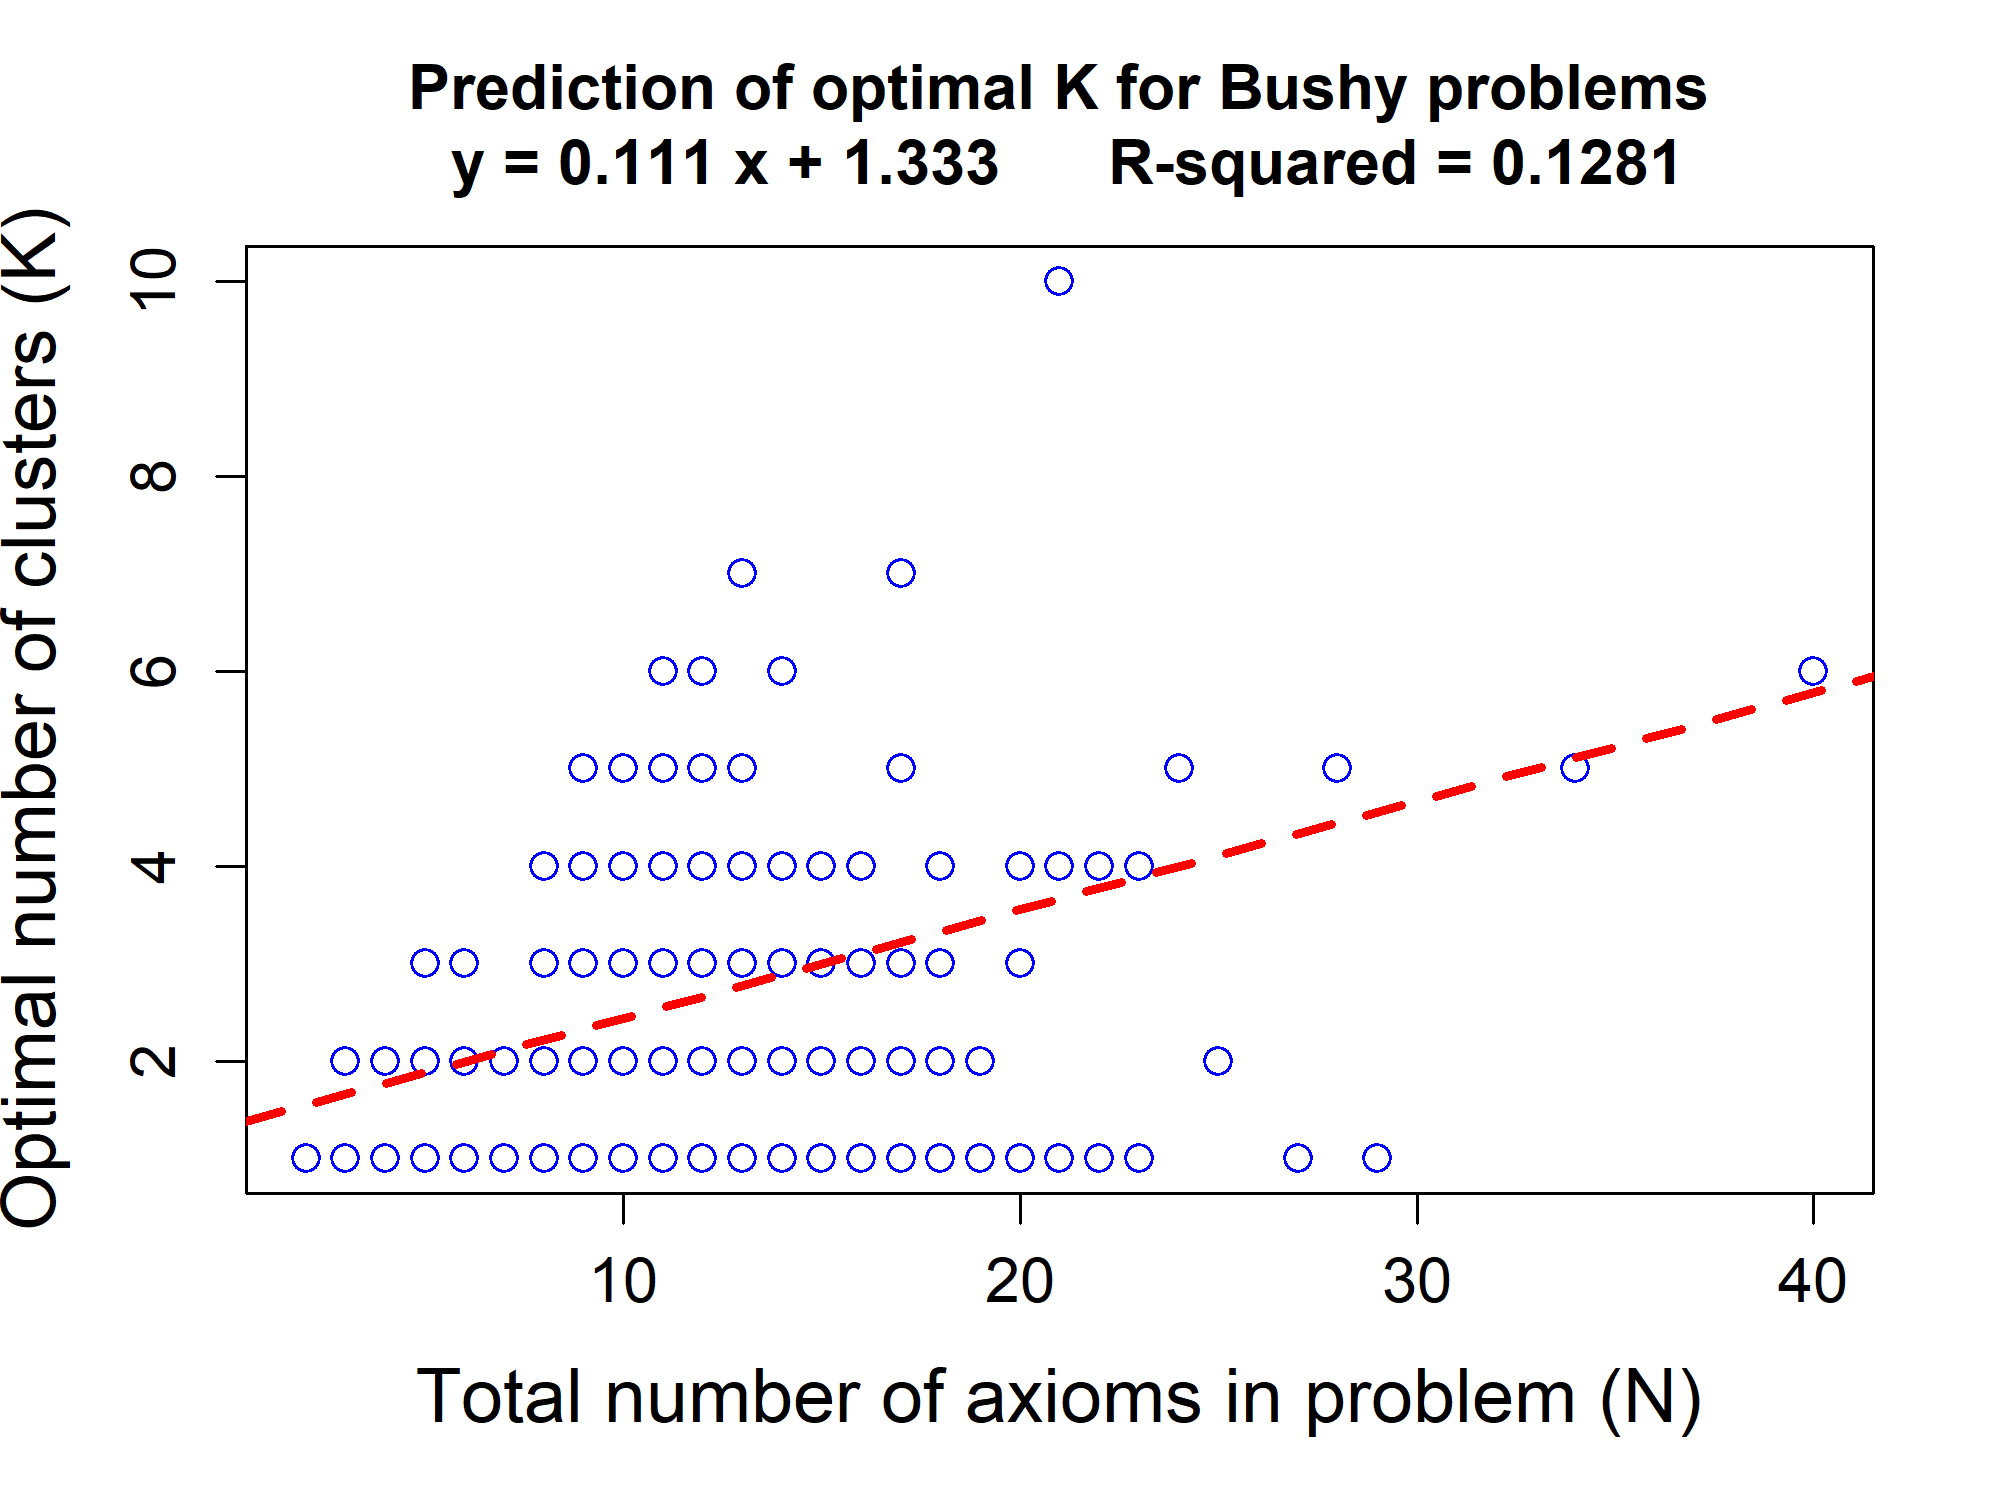
\includegraphics[scale=0.34]{median-regression-optimal-k-bushy.png}
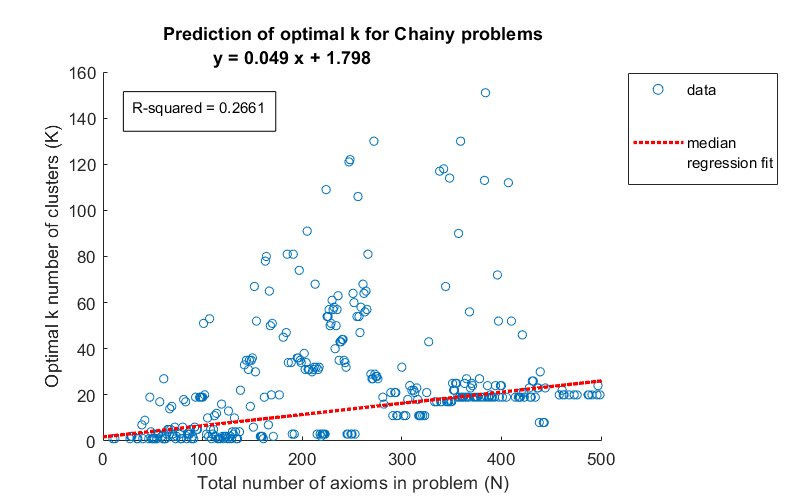
\includegraphics[scale=0.34]{median-regression-optimal-k-chainy.png}
\end{figure}

%------------------------------------------------------------------------------
\section{Evaluation Results}
\label{Results}

Section on evaluation
1. The test set(s)... Should we add tptp based set?
2. The results
3. The conclusions

Data on MPTPTP2078, Number of problems in test set, how selected (proofs,
hence already solved, but possibly with axiom selection), numbers of
different adequate subsets, average ratio nntp/all

%------------------------------------------------------------------------------
\section{Conclusion}
\label{Conclusion}

GEOFF:
1. Future correlate metrics with ptover performance (or do now!)

%------------------------------------------------------------------------------
\label{sect:bib}
\bibliographystyle{plain}
\bibliography{Bibliography}
%------------------------------------------------------------------------------
\end{document}
%------------------------------------------------------------------------------

